%!TEX root = ../report.tex

\begin{document}
    \chapter{Solution}

   \section{Hand crafted feature extraction}  
   First approach to analyze and explore the domain knowledge of the raw signal from accelerometer is calculating temporal, spectral and statistical aspects of the data. As discussed in chapter 3 domain specific knowledge can be extracted from time-series data to analyze it and used as input to machine learning algorithms as raw signal cannot be used directly. Along with the calculated features we have prior information that has been extracted from the signal that is, penetration and maximum velocity. The dataset contains three signals acceleration, velocity and position that are passed to feature extractor which extracts fixed set of features. Figure \ref{n0} shows example of set of features that have been extracted.
   
   \begin{figure}[h]
   	\centering
   	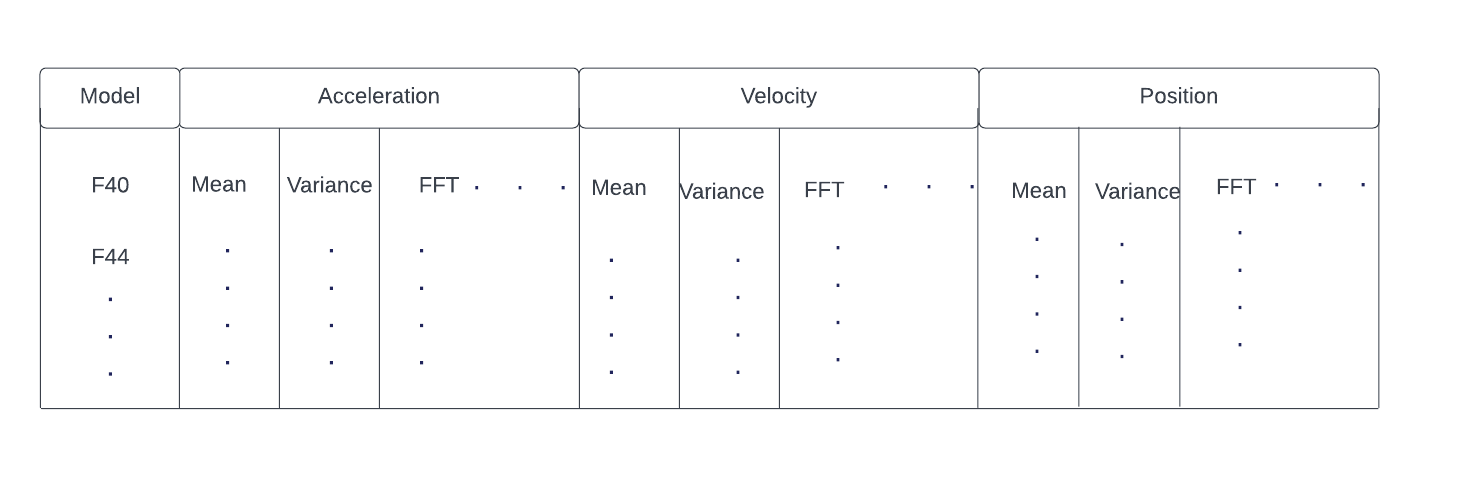
\includegraphics[width=1\linewidth]{images/featable.png}
   	\caption{Handcrafted features }
   	\label{n0}
   \end{figure}
   
   \begin{table}[h]
   	\centering
   	\begin{tabular}{|l|l|}
   		\hline
   		Type    & Features                                                                                                                                                                      \\ \hline
   		Statistical & \begin{tabular}[c]{@{}l@{}}Minimum, Maximum, Median, Mean absolute deviation, \\ Median absolute deviation, \\ Root mean square, Standard deviation, \\ Variance\end{tabular} \\ \hline
   		Temporal    & \begin{tabular}[c]{@{}l@{}}Mean absolute differences, Mean differences, \\ Median differences, Median absolute differences,\\  Entropy\end{tabular}                           \\ \hline
   		Spectral    & \begin{tabular}[c]{@{}l@{}}FFT mean coefficient, Minimum frequency, \\ Maximum frequency, Median frequency, \\ Fundamental frequency\end{tabular}                             \\ \hline
   	\end{tabular}
   	\caption{Fixed set of hand crafted features}
   	\label{t1}
   \end{table}
   
   
   
   The extractor function returns in total 54 features for each car door instance. Table \ref{t1} gives the overview of features calculated for each signal. The dimensionality of the feature vector obtained for each signal is reduced by removing the redundant features and selecting relevant ones by use of Random forest algorithm. This information is passed to supervised machine learning algorithm for classification.
   
   \section{Autoencoder for anomaly detection}   
   To apply a general classification approach there is a requirement of fixed number of classes to separate the data. The problem that is solved by this project contains two classes normal and abnormal. Proper definition of what distinct feature that can classify the signals into these classes is missing. In other words prior information on to what can be called as anomaly is not available because the data we are dealing with is a complex industrial dataset.  Also the data that is provided is highly imbalanced which has been seen during the data analysis in section $4.2.1$. Therefore a direct implementation of deep-learning algorithm to this problem is difficult. These problems arise when we try to find a classification algorithm to solve the problem. To overcome these issues we propose to re frame the problem as anomaly detection using autoencoder.
   
    \begin{figure}[h]
    	\centering
    	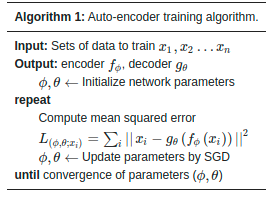
\includegraphics[width=0.5\linewidth]{images/algau.png}
    	\caption{Algorithm for anomaly detection \cite{oh2018residual} }
    	\label{n0}
    \end{figure}
   
   \section{Transfer learning with raw signal data}
   
   
   \section{Autoencoder as feature extractor}    
   
   
   \section{Transfer learning with spectrogram}   
\end{document}
